\documentclass[conference]{IEEEtran}
\usepackage[utf8]{inputenc}
\usepackage[T1]{fontenc}
\usepackage{lmodern}
\usepackage[brazil]{babel}
\usepackage{graphicx}
\usepackage{booktabs}
\usepackage{amsmath}
\usepackage{cite}
\usepackage{url}
\usepackage{microtype}
% GERADO por scripts/make_report_assets.py — não editar
\newcommand{\nTotal}{7692}
\newcommand{\nUnique}{7678}
\newcommand{\nDup}{14}
\newcommand{\nTrain}{5484}
\newcommand{\nVal}{1097}
\newcommand{\nTest}{1097}
\newcommand{\nGroups}{3956}
\newcommand{\nGrouped}{4918}
\newcommand{\nPlantDoc}{586}
\newcommand{\nSym}{180}
\newcommand{\accMajority}{24,8}
\newcommand{\accRGB}{60,4}
\newcommand{\accClassic}{96,7}
\newcommand{\accFinal}{95,1}
\newcommand{\accMobile}{97,6}
\newcommand{\fMobile}{97,5}
\newcommand{\ciMobile}{[96,6; 98,5]}
\newcommand{\selectedHead}{LogReg C=0.1 + aumento de dados (2 cópias)}
\newcommand{\nlpLR}{82,8}
\newcommand{\nlpSVM}{83,9}
\newcommand{\nlpLRci}{[77,2; 87,8]}
\newcommand{\nlpSVMci}{[78,3; 88,9]}
\newcommand{\intentAcc}{84,7}
\newcommand{\nIntent}{150}
\newcommand{\pdAcc}{43,9}
\newcommand{\pdCI}{[39,8; 48,0]}
\newcommand{\pdConf}{90,6}
\newcommand{\pvConf}{98,2}
\newcommand{\pdHalfNo}{45,4}
\newcommand{\pdHalfYes}{56,7}
\newcommand{\nPDhalf}{293}
\newcommand{\nPV}{1097}
\newcommand{\accVisPV}{95,3}
\newcommand{\covVisPV}{96,4}
\newcommand{\selVisPV}{98,8}
\newcommand{\accNlpPV}{76,3}
\newcommand{\covNlpPV}{87,6}
\newcommand{\selNlpPV}{87,1}
\newcommand{\accIntPV}{87,7}
\newcommand{\covIntPV}{88,3}
\newcommand{\selIntPV}{99,3}
\newcommand{\sensIntPVTen}{79,0}
\newcommand{\sensSelPVTen}{99,1}
\newcommand{\sensIntPVThirty}{62,9}
\newcommand{\sensSelPVThirty}{99,0}
\newcommand{\divPctPV}{11,1}
\newcommand{\nPD}{586}
\newcommand{\accVisPD}{39,9}
\newcommand{\covVisPD}{83,8}
\newcommand{\selVisPD}{47,7}
\newcommand{\accNlpPD}{77,6}
\newcommand{\covNlpPD}{89,8}
\newcommand{\selNlpPD}{86,5}
\newcommand{\accIntPD}{42,5}
\newcommand{\covIntPD}{48,5}
\newcommand{\selIntPD}{87,7}
\newcommand{\sensIntPDTen}{38,7}
\newcommand{\sensSelPDTen}{85,0}
\newcommand{\sensIntPDThirty}{32,2}
\newcommand{\sensSelPDThirty}{80,1}
\newcommand{\divPctPD}{51,4}


\begin{document}

\title{PlantAI: Sistema Multiagente com Visão Computacional e PLN para Apoio ao Diagnóstico de Doenças Foliares em Tomate, Batata e Milho}

\author{\IEEEauthorblockN{Lucas Gomes, Viny Carnaúba, Fabiano Nasiazeno, José Nogueira e Marco Wichmann}
\IEEEauthorblockA{AFYA | UNIMA Maceió --- Disciplina de Inteligência Artificial (Prof. Ícaro Ferreira)\\
Código: \texttt{https://github.com/lucazcoding/plantAI}}}

\date{}
\maketitle

\begin{abstract}
Este trabalho apresenta o PlantAI, um sistema multiagente que recebe a foto de uma folha e uma mensagem em português (sintomas e pergunta) e responde com diagnóstico, tratamento, prevenção ou gravidade. A visão usa um MobileNetV2 pré-treinado no ImageNet, com características multiescala e cabeça supervisionada treinada em imagens reais do PlantVillage (6 classes de tomate, batata e milho); o PLN classifica sintomas (TF-IDF) e reconhece a intenção da pergunta; seis regras explícitas fundem as evidências. A avaliação usa divisão 71/14/14\% agrupada por folha, para evitar vazamento. No teste do PlantVillage (N=\nTest) a cabeça atinge \accMobile\% de acurácia, contra \accRGB\% de um baseline RGB. Em fotos de campo do PlantDoc (N=\nPlantDoc), porém, a acurácia cai para \pdAcc\%, e a confiança média (\pdConf\%) mostra que as probabilidades não são calibradas fora do domínio. A fusão visão+texto troca cobertura por confiabilidade: em campo, a precisão das respostas sobe de \selVisPD\% para \selIntPD\% com cobertura de \covIntPD\%. Os resultados são reais e reproduzíveis; as limitações são discutidas.
\end{abstract}

\begin{IEEEkeywords}
doenças de plantas, visão computacional, PLN, sistemas multiagente, transfer learning, PlantVillage.
\end{IEEEkeywords}

\section{Introdução}
Doenças foliares reduzem a produtividade de culturas como tomate, batata e milho, e o diagnóstico precoce depende de especialistas nem sempre disponíveis ao produtor. Classificadores de imagens treinados no PlantVillage \cite{hughes2015,mohanty2016} reportam acurácias acima de 98\%, mas esses números são obtidos em imagens de laboratório com fundo homogêneo e podem superestimar o desempenho em campo \cite{noyan2022,singh2020}.

O objetivo deste trabalho é construir e avaliar, de forma reproduzível, uma aplicação que integre Machine Learning, Visão Computacional e Processamento de Linguagem Natural (PLN) no mesmo fluxo: o usuário envia uma imagem e faz uma pergunta; a visão extrai evidências da imagem; o PLN interpreta o relato e a pergunta; um componente de decisão combina os resultados e responde. As contribuições são: (i) a arquitetura multiagente com seis regras de decisão auditáveis; (ii) uma avaliação com dados reais, divisão sem vazamento por folha e intervalos de confiança; (iii) uma análise honesta da generalização para fotos de campo e do efeito da fusão visão+texto.

\section{Fundamentação e Trabalhos Relacionados}
\textbf{Dados.} O PlantVillage reúne mais de 54 mil imagens de folhas saudáveis e doentes \cite{hughes2015}; Mohanty et al.\ treinaram redes profundas nele e observaram queda de desempenho em imagens de outras fontes \cite{mohanty2016}. Noyan mostrou que apenas 8 pixels do fundo bastam para um classificador atingir 49\% de acurácia, evidenciando viés de captura \cite{noyan2022}. O PlantDoc oferece imagens obtidas na web, com fundos e iluminação variados \cite{singh2020}.

\textbf{Transfer learning.} O MobileNetV2 \cite{sandler2018}, treinado no ImageNet \cite{deng2009}, fornece representações reutilizáveis. Neste trabalho o backbone fica congelado e uma cabeça é treinada sobre suas ativações.

\textbf{PLN e decisão.} A classificação de sintomas usa TF-IDF \cite{salton1988} com modelos lineares do scikit-learn \cite{pedregosa2011}. A decisão segue a ideia de agentes baseados em regras \cite{russell2020}: cada regra é explícita, testável e registra a evidência usada.

\section{Metodologia}
\subsection{Arquitetura}
A Fig.~\ref{fig:arq} mostra o fluxo. O \textit{CoordinatorAgent} separa a mensagem em relato de sintomas e pergunta; o \textit{VisionAgent} valida a imagem (integridade, brilho, nitidez), redimensiona para $224{\times}224$ e extrai características; o \textit{MLAgent} classifica; o \textit{NLPAgent} classifica o relato e um segundo modelo reconhece a intenção da pergunta (diagnóstico, tratamento, prevenção, gravidade, confirmação). O \textit{DecisionRulesEngine} aplica seis regras: R1 rejeição por qualidade de imagem; R2 modo somente visual ou somente texto; R3 concordância com reforço de confiança; R4 desempate textual quando a visão tem confiança moderada; R5 divergência explícita (o sistema se abstém e mostra as hipóteses); R6 incerteza geral. Os agentes se comunicam por um contrato tipado (classe, confiança, top-$k$, metadados).

\begin{figure}[t]\centering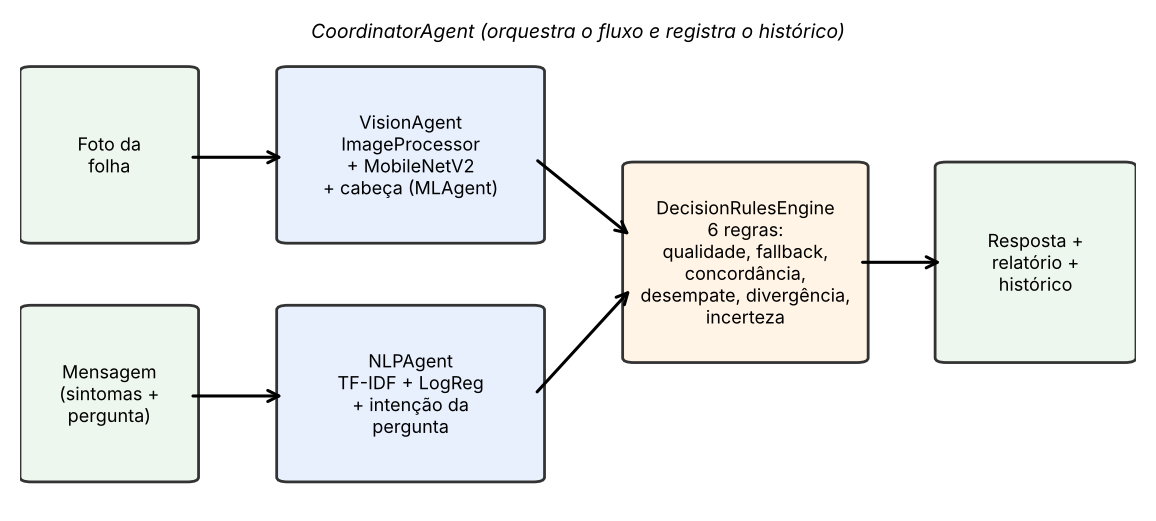
\includegraphics[width=\columnwidth]{figuras/arquitetura.png}\caption{Arquitetura multiagente do PlantAI.}\label{fig:arq}\end{figure}

\subsection{Dados e preparação}
\textbf{PlantVillage} (CC BY-SA 3.0): as seis classes do projeto, com \nTotal{} imagens coloridas; após remover \nDup{} duplicatas exatas (MD5) e arquivos ilegíveis (nenhum), restaram \nUnique{}. O PlantVillage fotografa a mesma folha em várias orientações; por isso a divisão usa \textit{StratifiedGroupKFold} com o mapa folha$\to$imagem de Mohanty et al.\ (disponível para \nGrouped{} imagens; as demais são tratadas como independentes), resultando em \nTrain{}/\nVal{}/\nTest{} imagens para treino/validação/teste, sem folha compartilhada entre partições (verificado por teste automatizado). \textbf{PlantDoc} (CC BY 4.0): \nPlantDoc{} imagens de campo das mesmas classes, usadas \emph{apenas} para avaliação externa (e para um experimento de adaptação, abaixo).

\textbf{Textos.} Um corpus de \nSym{} descrições de sintomas, redigido pela equipe (30 por classe, em estilos técnico, coloquial, curto e com erros de digitação; parte sem citar a cultura), e \nIntent{} perguntas rotuladas por intenção.

\subsection{Modelos e protocolo}
\textbf{Visão.} O backbone é o MobileNetV2 1.0/224 do ImageNet, quantizado em INT8 (TensorFlow Lite) e executado em CPU. Comparam-se: classe majoritária; 6 estatísticas RGB + regressão logística; 30 descritores clássicos (cor, índices de verde, razões de lesão, textura) + MLP; e o MobileNetV2 com a cabeça treinada sobre (a) o vetor global de 1280 dimensões ou (b) esse vetor concatenado à média e ao desvio das ativações de quatro blocos intermediários (1984 dimensões). A representação, a cabeça (regressão logística, $C\in[10^{-4},10]$, ou MLP) e o uso de aumento de dados no treino (recorte, giro, rotação, cor, desfoque) foram escolhidos na \emph{validação}; o teste só foi lido ao final. O modelo implantado é: \selectedHead.

\textbf{PLN.} TF-IDF (uni+bigramas) com regressão logística ou LinearSVC calibrado, avaliados por validação cruzada 5-fold; as predições de cada texto vêm sempre de um modelo que não o viu. Reportam-se duas variantes: o pipeline TF-IDF + modelo linear \emph{puro} e o \textit{NLPAgent} implantado, que acrescenta uma regra auditável: quando exatamente uma cultura é citada no texto, as probabilidades das classes dessa cultura são multiplicadas por 1,35 e as demais por 0,75, com renormalização.

\textbf{Integração (Exp.~5).} Cada imagem é pareada com um texto sorteado da mesma classe (predição fora da dobra do PLN), supondo um usuário que descreve corretamente o que vê; uma varredura troca uma fração $p$ dos textos por textos de outra classe, simulando erro do usuário. Comparam-se visão isolada, PLN isolado e sistema integrado. Como o sistema pode se abster, reportam-se acurácia estrita (abstenção conta como erro), cobertura e precisão entre as respondidas. Intervalos de 95\% usam bootstrap (2000 reamostragens). Semente 42; ambiente em \texttt{results/metrics/environment.json}.

\section{Resultados e Discussão}
\subsection{Visão em laboratório}
A Tabela~\ref{tab:vis} resume o teste do PlantVillage. A cabeça sobre o MobileNetV2 multiescala atinge \accMobile\% (IC95\% \ciMobile), contra \accFinal\% com o vetor global e \accRGB\% do baseline RGB. Um resultado relevante é que 30 descritores clássicos já chegam a \accClassic\%: no PlantVillage, atributos simples de cor e textura separam bem as classes, coerente com o viés de captura descrito em \cite{noyan2022}. Assim, a acurácia em laboratório não prova que o modelo ``entende'' a doença. Os erros residuais concentram-se entre pinta-preta e requeima do tomate e entre requeima de batata e de tomate (Fig.~\ref{fig:cm}).

% GERADO por scripts/make_report_assets.py
\begin{table}[t]\caption{Modelos visuais no conjunto de teste do PlantVillage (N=1097). IC 95\% por bootstrap.}\label{tab:vis}\centering\small
\resizebox{\columnwidth}{!}{\begin{tabular}{lcc}\toprule Modelo & Acurácia (\%) & F1-macro (\%)\\\midrule
Classe majoritária & 24,8 & 6,6\\
6 estatísticas RGB + LogReg & 60,4 & 62,2\\
30 descritores clássicos + MLP & 96,6 & 96,5\\
MobileNetV2 (1280-d final) + LogReg & 95,1 & 95,0\\
MobileNetV2 multiescala + cabeça (implantado) & 97,6 & 97,5\\
\bottomrule\end{tabular}}\end{table}
\begin{table}[t]\caption{PLN: validação cruzada 5-fold (textos avaliados fora da dobra). ``Puro'' = TF-IDF + modelo linear; ``regra de cultura'' = reforço $\times$1,35/$\times$0,75 do NLPAgent.}\label{tab:nlp}\centering\small
\resizebox{\columnwidth}{!}{\begin{tabular}{lccc}\toprule Modelo & N & Acurácia (\%) & F1-macro (\%)\\\midrule
TF-IDF + LogReg (puro) & 180 & 80,6 & 80,6\\
TF-IDF + SVC calibrado (puro) & 180 & 81,1 & 81,2\\
NLPAgent: LogReg + regra de cultura & 180 & 82,8 & 82,8\\
NLPAgent: SVC + regra de cultura & 180 & 83,9 & 83,9\\
Intenção da pergunta (LogReg) & 150 & 84,7 & 84,7\\\bottomrule\end{tabular}}\end{table}
\begin{table*}[t]\caption{Experimento 5 -- ablação (texto correto). Acurácia estrita conta \textit{inconclusivo} como erro; cobertura = fração respondida; precisão = acurácia entre as respondidas.}\label{tab:abl}\centering\small
\resizebox{\textwidth}{!}{\begin{tabular}{llccc}\toprule Conjunto & Modo & Acurácia estrita (\%) & Cobertura (\%) & Precisão se respondeu (\%)\\\midrule
PlantVillage teste (N=1097) & Visão isolada & 95,3 & 96,4 & 98,8\\
PlantVillage teste (N=1097) & PLN isolado & 76,3 & 87,6 & 87,1\\
PlantVillage teste (N=1097) & Integrado (visão+PLN+regras) & 87,5 & 88,0 & 99,5\\
\midrule
PlantDoc campo (N=586) & Visão isolada & 39,9 & 83,8 & 47,7\\
PlantDoc campo (N=586) & PLN isolado & 77,6 & 89,8 & 86,5\\
PlantDoc campo (N=586) & Integrado (visão+PLN+regras) & 40,8 & 46,4 & 87,9\\
\bottomrule\end{tabular}}\end{table*}
\begin{table}[t]\caption{Generalização de domínio (acurácia, \%).}\label{tab:dom}\centering\small
\resizebox{\columnwidth}{!}{\begin{tabular}{lc}\toprule Cenário & Acurácia\\\midrule
PlantVillage, teste (N=1097) & 97,6\\
PlantDoc todo (N=586) & 43,9\\
PlantDoc 50\% (N=293), sem adapt. & 43,0\\
PlantDoc 50\%, com adapt. & 57,3\\\bottomrule\end{tabular}}\end{table}


\begin{figure}[t]\centering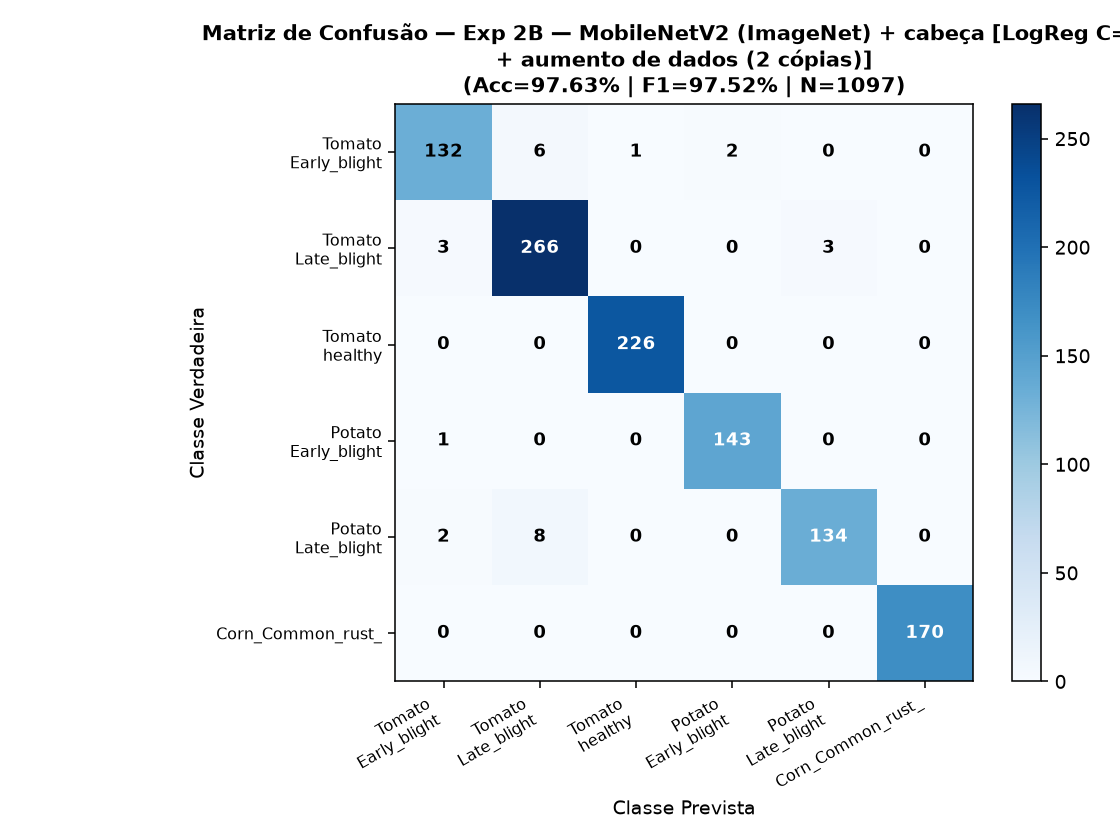
\includegraphics[width=0.9\columnwidth]{figuras/cm_visao.png}\caption{Matriz de confusão do modelo implantado no teste do PlantVillage.}\label{fig:cm}\end{figure}

\subsection{PLN}
Na Tabela~\ref{tab:nlp}, o pipeline TF-IDF puro obtém \nlpLRpure\% (regressão logística) e \nlpSVMpure\% (SVM). Com o reforço por cultura citada, que faz parte do \textit{NLPAgent} e dos experimentos de integração, os valores sobem para \nlpLR\% (IC95\% \nlpLRci) e \nlpSVM\% (IC95\% \nlpSVMci); o ganho de cerca de 2 a 3 pontos vem da regra, não do modelo linear, e deve ser lido assim. O principal erro é confundir tomate e batata em textos que descrevem a lesão sem citar a cultura, pois o texto realmente não distingue as espécies; a imagem resolve essa ambiguidade. A intenção da pergunta é reconhecida com \intentAcc\% de acurácia em \nIntent{} perguntas.

\subsection{Integração visão+texto}
A Tabela~\ref{tab:abl} e a Fig.~\ref{fig:abl} mostram a ablação. No PlantVillage, a visão responde \covVisPV\% dos casos com precisão de \selVisPV\%; o sistema integrado responde \covIntPV\% com precisão de \selIntPV\%. Sua acurácia estrita (\accIntPV\%) é \emph{menor} que a da visão (\accVisPV\%) porque divergências entre imagem e texto (\divPctPV\% dos casos, coerente com a precisão de \selNlpPV\% do PLN isolado) levam à abstenção (R5). Em campo, a visão acerta apenas \accVisPD\% e, ao responder, tem precisão de \selVisPD\%; o integrado responde \covIntPD\% dos casos com precisão de \selIntPD\%. Portanto, a fusão não aumenta a acurácia bruta, mas funciona como filtro de confiabilidade: a divergência sinaliza justamente onde a visão erra com alta confiança. Esse ganho depende da qualidade do relato: com 30\% dos textos trocados por outra classe, a precisão do integrado cai para \sensSelPDThirty\% em campo (e permanece em \sensSelPVThirty\% no PlantVillage), enquanto a cobertura diminui (Fig.~\ref{fig:sens}).

\begin{figure}[t]\centering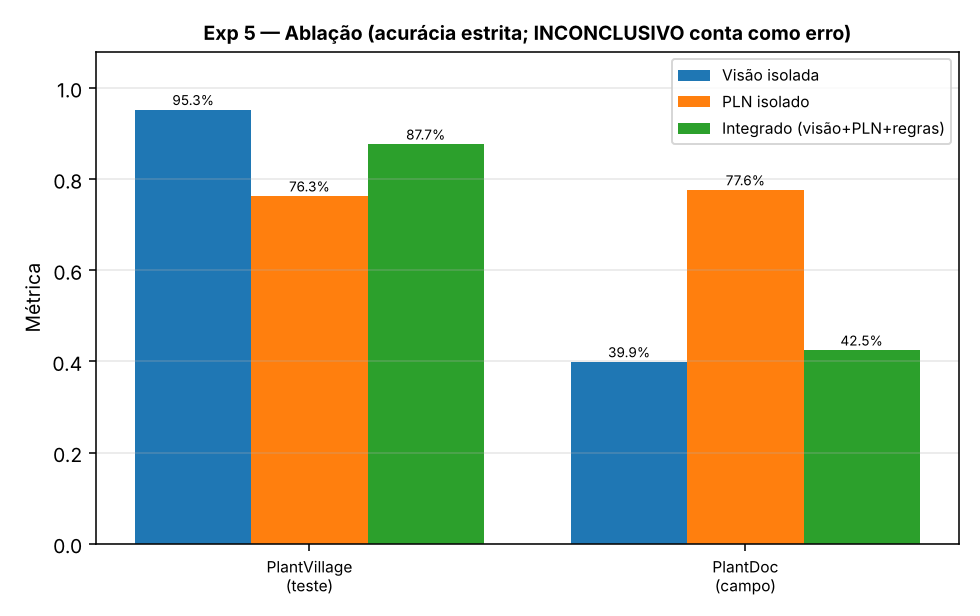
\includegraphics[width=\columnwidth]{figuras/ablacao.png}\caption{Ablação (acurácia estrita).}\label{fig:abl}\end{figure}

\subsection{Generalização para campo e adaptação}
A Tabela~\ref{tab:dom} mostra a queda de \accMobile\% para \pdAcc\% (IC95\% \pdCI) no PlantDoc. A confiança média do modelo é \pdConf\% em campo e \pvConf\% no teste do PlantVillage: as probabilidades não são calibradas fora do domínio, o que limita o uso dos limiares de confiança das regras. Treinar com metade do PlantDoc eleva a acurácia na outra metade de \pdHalfNo\% para \pdHalfYes\% (N=\nPDhalf), indicando que dados de campo são o caminho mais promissor.

\begin{figure}[t]\centering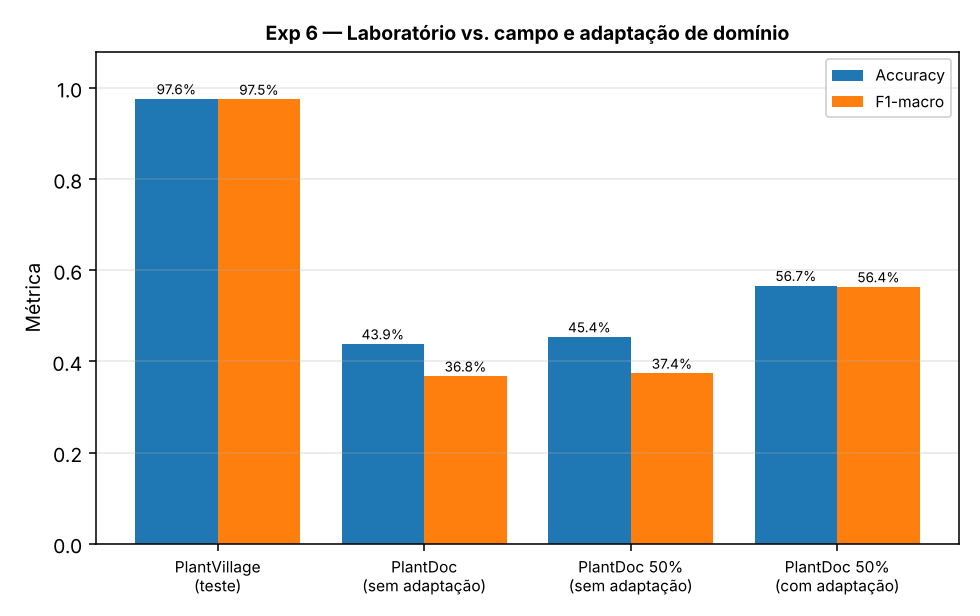
\includegraphics[width=\columnwidth]{figuras/dominio.png}\caption{Laboratório vs.\ campo e adaptação de domínio.}\label{fig:dom}\end{figure}
\begin{figure}[t]\centering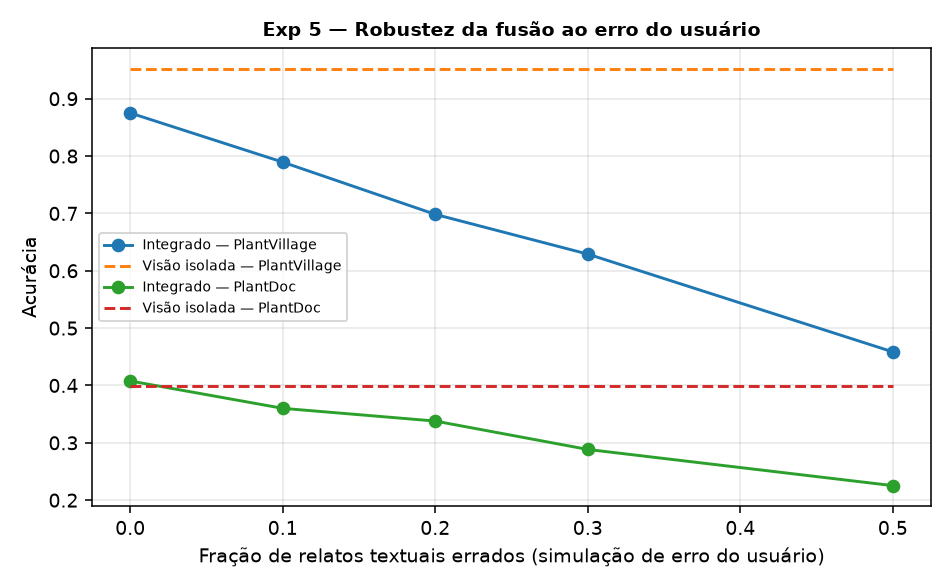
\includegraphics[width=0.85\columnwidth]{figuras/sensibilidade.png}\caption{Robustez do sistema integrado ao erro do usuário (texto trocado por outra classe).}\label{fig:sens}\end{figure}

\subsection{Limitações}
(i) O backbone está congelado e quantizado; o \textit{fine-tuning} completo (script para Colab no repositório) não foi executado neste trabalho. (ii) O mapa de folhas cobre \nGrouped{} das \nUnique{} imagens; fotos sem mapeamento podem ainda ser quase duplicatas entre partições. (iii) O PlantVillage tem viés de fundo e captura \cite{noyan2022}. (iv) Os textos foram redigidos pela equipe e, no Exp.~5, são sorteados da classe verdadeira; é um cenário otimista, mitigado apenas pela varredura de erro. (v) O PlantDoc é pequeno e ruidoso. (vi) O aumento de dados foi incluído depois de observarmos o baixo desempenho em campo; a regra de adoção (validação a até 1 p.p. da melhor) foi fixada antes da execução final e o efeito é pequeno. (vii) Não houve avaliação com usuários nem validação por agrônomos; o sistema não substitui diagnóstico profissional.

\section{Conclusão e Trabalhos Futuros}
O PlantAI integra visão, ML, PLN e regras em um fluxo imagem+pergunta$\to$resposta, com resultados reais: \accMobile\% no PlantVillage, mas \pdAcc\% em fotos de campo. A fusão visão+texto aumenta a precisão das respostas ao custo de cobertura. Trabalhos futuros: \textit{fine-tuning} completo com aumento forte e dados de campo, calibração de probabilidades, textos coletados de produtores reais, mais culturas e validação com agrônomos.

\begin{thebibliography}{10}
\bibitem{hughes2015} D.~P. Hughes and M.~Salath\'e, ``An open access repository of images on plant health to enable the development of mobile disease diagnostics,'' arXiv:1511.08060, 2015.
\bibitem{mohanty2016} S.~P. Mohanty, D.~P. Hughes, and M.~Salath\'e, ``Using deep learning for image-based plant disease detection,'' \textit{Frontiers in Plant Science}, vol.~7, p.~1419, 2016, doi:10.3389/fpls.2016.01419.
\bibitem{singh2020} D.~Singh \textit{et al.}, ``PlantDoc: A dataset for visual plant disease detection,'' in \textit{Proc. CoDS-COMAD}, 2020, pp.~249--253, doi:10.1145/3371158.3371196.
\bibitem{noyan2022} M.~A. Noyan, ``Uncovering bias in the PlantVillage dataset,'' arXiv:2206.04374, 2022.
\bibitem{sandler2018} M.~Sandler \textit{et al.}, ``MobileNetV2: Inverted residuals and linear bottlenecks,'' in \textit{Proc. IEEE CVPR}, 2018, pp.~4510--4520.
\bibitem{deng2009} J.~Deng \textit{et al.}, ``ImageNet: A large-scale hierarchical image database,'' in \textit{Proc. IEEE CVPR}, 2009, pp.~248--255.
\bibitem{salton1988} G.~Salton and C.~Buckley, ``Term-weighting approaches in automatic text retrieval,'' \textit{Inf. Process. Manage.}, vol.~24, no.~5, pp.~513--523, 1988.
\bibitem{pedregosa2011} F.~Pedregosa \textit{et al.}, ``Scikit-learn: Machine learning in Python,'' \textit{J. Mach. Learn. Res.}, vol.~12, pp.~2825--2830, 2011.
\bibitem{russell2020} S.~Russell and P.~Norvig, \textit{Artificial Intelligence: A Modern Approach}, 4th ed. Pearson, 2020.
\end{thebibliography}
\end{document}
